\section{Parte 3: Registro de Estimaciones}

\subsection{Registro y Configuración en Jira Software}

Una vez alcanzado el consenso en la sesión de Planning Poker, se procedió a asentar los resultados dentro del proyecto oficial de Jira Software (\textbf{Proyecto \texttt{SC} -- SIGC-CUSCO}). Para garantizar la máxima trazabilidad operativa y el control visual del progreso, se configuraron los siguientes elementos en cada tarjeta:

\begin{enumerate}
    \item \textbf{Campo numérico nativo de estimación:} Se ingresó el puntaje acordado en el campo estándar \texttt{Story point estimate} de Jira, permitiendo que la plataforma calcule automáticamente la velocidad del equipo y el peso de los sprints.
    \item \textbf{Etiquetas semánticas de clasificación:} Con el objetivo de filtrar y generar vistas agrupadas de manera instantánea, se incorporaron etiquetas estandarizadas:
    \begin{itemize}
        \item Por tamaño relativo: \texttt{sp-corta}, \texttt{sp-media} y \texttt{sp-compleja}.
        \item Por alcance de práctica: \texttt{lab05}.
        \item Por prioridad de negocio: \texttt{moscow-must}, \texttt{moscow-should} y \texttt{moscow-could}.
        \item Para trazabilidad de refactorización ágil: \texttt{dividida} (para las historias padre complejas) y \texttt{refinamiento} (para las historias hijas resultantes).
    \end{itemize}
    \item \textbf{Memoria técnica de votación:} En la descripción de cada issue o en su sección de comentarios, se dejó constancia formal de las rondas de votación registradas (ej. \enquote{Ronda 1: 5 / 13 / 8, Ronda 2: 8 / 13 / 13 $\rightarrow$ Consenso 13 SP}) y la justificación técnica resumida que sustentó la decisión del equipo.
\end{enumerate}

Las Figuras~\ref{fig:jira_backlog_p1} y~\ref{fig:jira_backlog_p2} presentan la vista general del Backlog en Jira Software, donde se aprecia la distribución de las historias de usuario, sus épicas asociadas y el puntaje asignado en la columna derecha.

\begin{figure}[H]
    \centering
    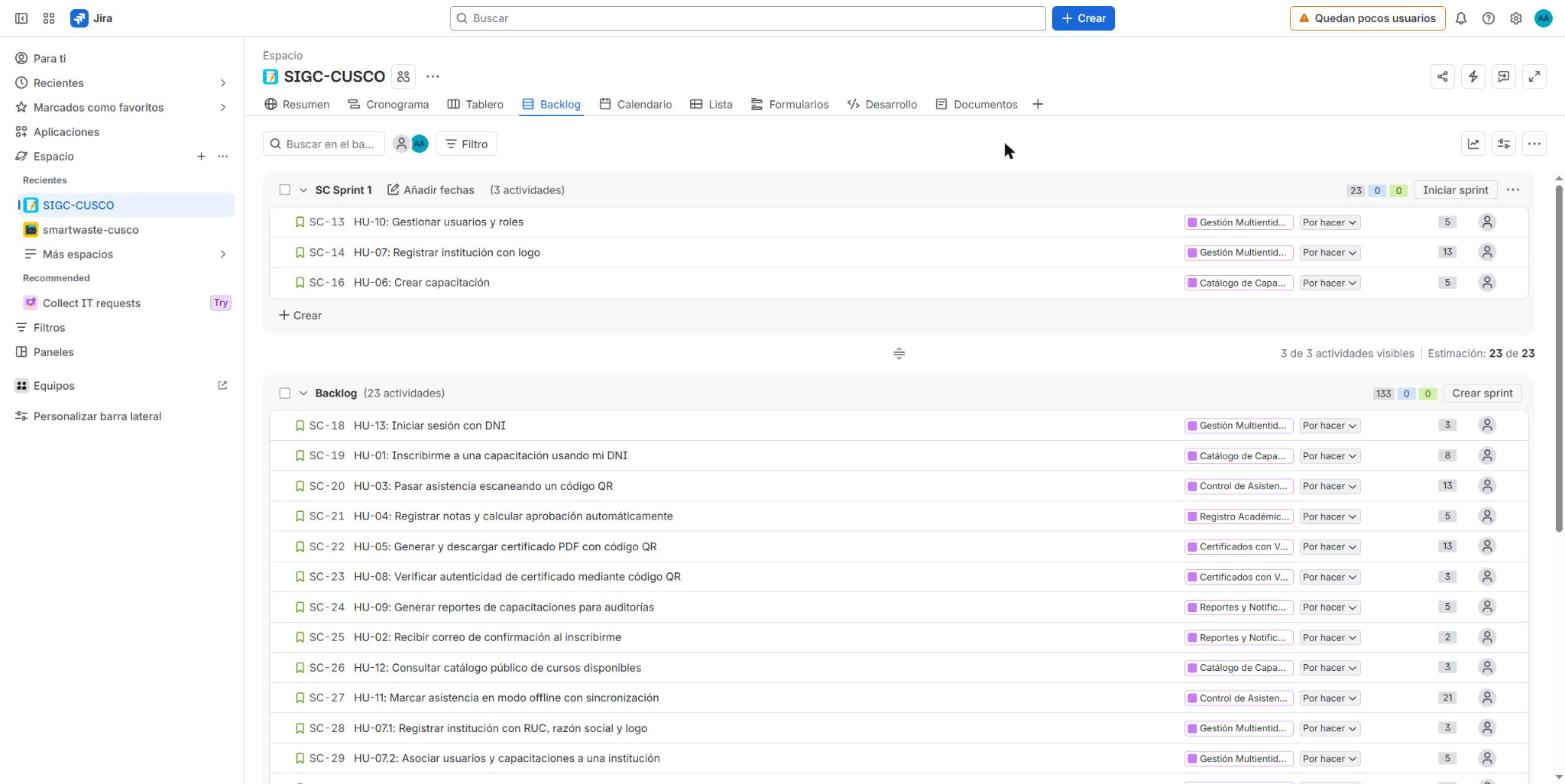
\includegraphics[width=\textwidth]{figura2_backlog_jira_parte1.jpg}
    \caption{Backlog del proyecto SC en Jira Software con la estimación en story points (columna derecha). Parte 1: SC Sprint 1 planificado y primeras historias del backlog general.}
    \label{fig:jira_backlog_p1}
\end{figure}

\begin{figure}[H]
    \centering
    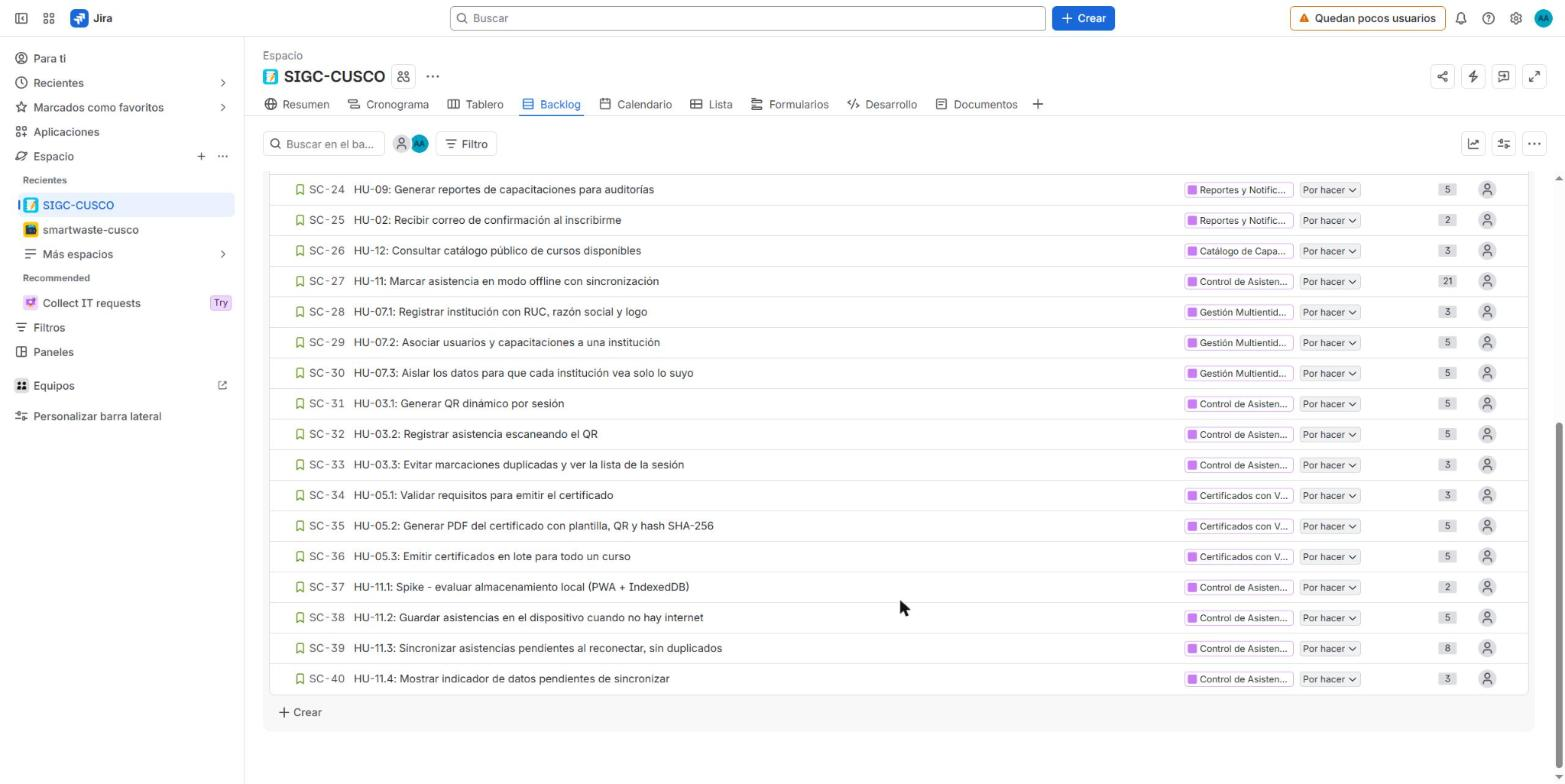
\includegraphics[width=\textwidth]{figura3_backlog_jira_parte2.jpg}
    \caption{Backlog en Jira Software, Parte 2: historias SC-24 a SC-40 (incluyendo las historias hijas refinadas). La columna de Story Points refleja la completitud del registro.}
    \label{fig:jira_backlog_p2}
\end{figure}

Para gestionar eficazmente las historias de gran envergadura que ponen en riesgo la predictibilidad de las iteraciones, se configuró el filtro de búsqueda avanzada JQL:
\begin{center}
    \texttt{project = SC AND labels = sp-compleja}
\end{center}
Dicha consulta extrae de forma inmediata los ítems que requieren descomposición obligatoria antes de ingresar al Sprint Planning. La Figura~\ref{fig:jira_detalle_sc20} muestra como ejemplo la tarjeta detallada de \textbf{SC-20 (HU-03)}, exhibiendo sus criterios de aceptación en formato BDD, el historial de votos documentado y las etiquetas asignadas.

\begin{figure}[H]
    \centering
    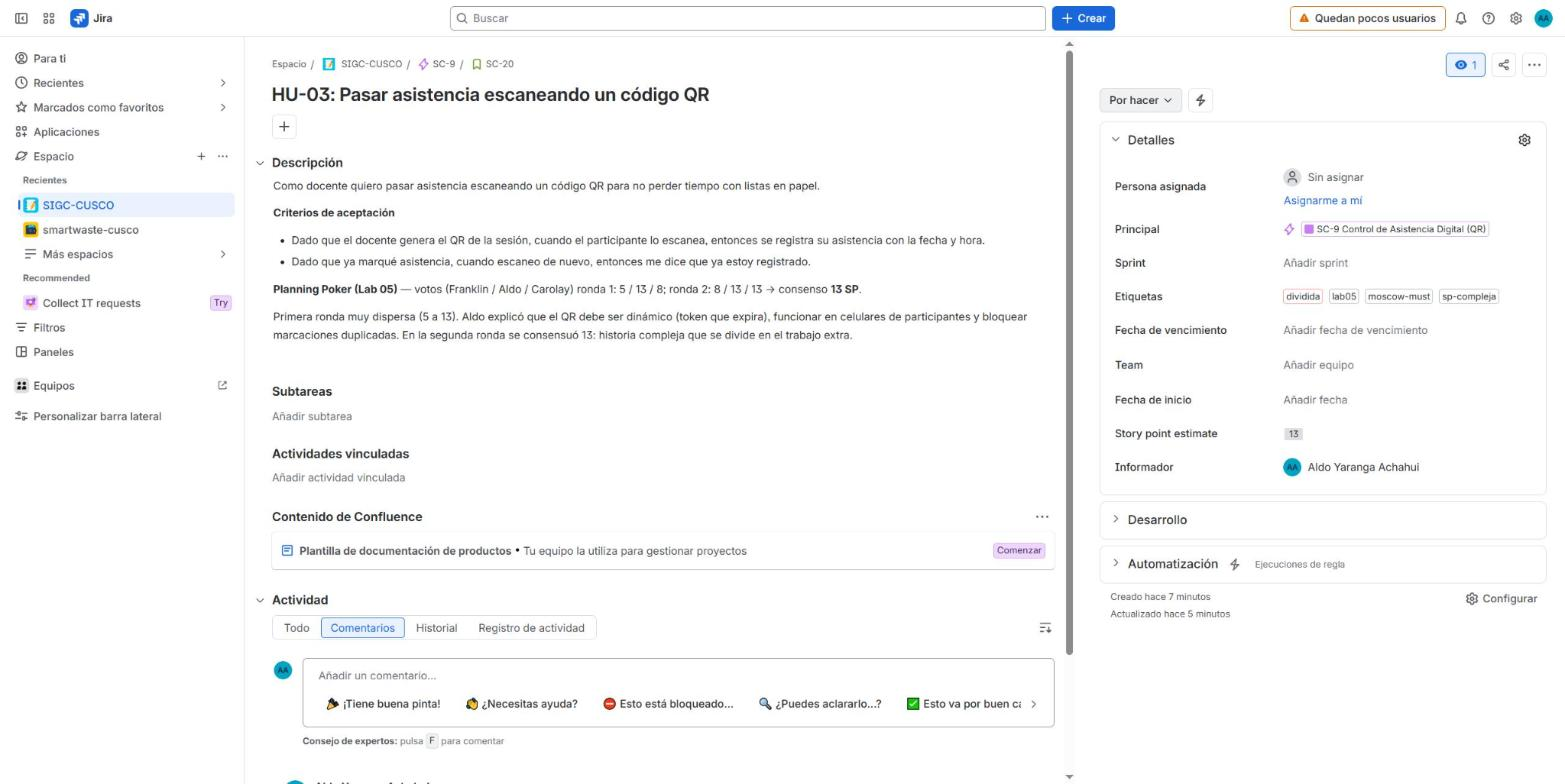
\includegraphics[width=\textwidth]{figura4_detalle_sc20_jira.jpg}
    \caption{Detalle de la historia SC-20 (HU-03) en Jira Software: votos de ambas rondas en la descripción, campo Story point estimate = 13 y etiquetas \texttt{sp-compleja}, \texttt{dividida}, \texttt{lab05} y \texttt{moscow-must}.}
    \label{fig:jira_detalle_sc20}
\end{figure}

\subsection{Clasificación de las Historias de Usuario por Tamaño}

De acuerdo con las directrices metodológicas de la guía de laboratorio, las historias de usuario fueron agrupadas en tres categorías según su puntaje de Fibonacci:
\begin{itemize}
    \item \textbf{Historias Cortas (1--3 SP):} Tareas atómicas de baja complejidad, con bajo riesgo y esfuerzo acotado (interfaces de consulta, notificaciones estándar o autenticación preconfigurada).
    \item \textbf{Historias Medias (5--8 SP):} Requerimientos que exigen lógica de negocio sustancial, transacciones con validación de integridad o reportería estructurada, pero cuya arquitectura es plenamente conocida por el equipo.
    \item \textbf{Historias Complejas (13+ SP):} Requerimientos de alta incertidumbre, dependencias externas críticas o arquitectura no trivial que no deben abordarse directamente en un sprint sin descomposición previa.
\end{itemize}

La Tabla~\ref{tab:clasificacion_historias} sintetiza el criterio de clasificación y la distribución estadística resultante en el backlog inicial del SIGC-CUSCO.

\begin{table}[H]
\centering
\small
\renewcommand{\arraystretch}{1.2}
\caption{Criterio de clasificación por tamaño y distribución estadística del backlog inicial.}
\label{tab:clasificacion_historias}
\begin{tabularx}{\textwidth}{P{2.2cm} C{2.2cm} C{2.2cm} C{2.0cm} Y}
\toprule
\rowcolor{headerblue}
\textcolor{white}{\textbf{Categoría}} & \textcolor{white}{\textbf{Rango}} & \textcolor{white}{\textbf{N° Historias}} & \textcolor{white}{\textbf{Suma SP}} & \textcolor{white}{\textbf{Historias Incluidas}} \\
\midrule
\rowcolor{white}
\textbf{Cortas} & 1--3 SP & 4 (30.8\%) & 11 SP (11.1\%) & HU-02, HU-08, HU-12, HU-13 \\
\rowcolor{rowalt}
\textbf{Medias} & 5--8 SP & 5 (38.5\%) & 28 SP (28.3\%) & HU-01, HU-04, HU-06, HU-09, HU-10 \\
\rowcolor{white}
\textbf{Complejas} & 13+ SP & 4 (30.8\%) & 60 SP (60.6\%) & HU-03, HU-05, HU-07, HU-11 \\
\midrule
\rowcolor{headerblue!10}
\textbf{Total Inicial} & -- & \textbf{13 historias} & \textbf{99 SP} & \textit{Concentración del 60.6\% del esfuerzo en complejas} \\
\bottomrule
\end{tabularx}
\end{table}

\textbf{Diagnóstico analítico de la distribución:}
El resultado inicial revela un síntoma clásico en la gestión de proyectos de software: aunque las historias complejas representan únicamente el $30.8\%$ del número de ítems (4 de 13), concentran más del \textbf{60\% del esfuerzo total del backlog} (60 de 99 SP). Introducir estas cuatro historias en su estado actual dentro de los sprints de desarrollo provocaría cuellos de botella en control de calidad, bloqueos imprevistos e incrementos de deuda técnica. Esta evidencia cuantitativa confirma la necesidad imperativa del refinamiento abordado en el trabajo extra.

\subsection{Entregable Oficial: Product Backlog con Estimaciones}

La Tabla~\ref{tab:product_backlog_estimado} presenta el Product Backlog formal del SIGC-CUSCO, ordenado estratégicamente por nivel de prioridad MoSCoW, integrando la clave Jira, código de historia, título descriptivo, épica, prioridad, valor en Story Points y su clasificación cualitativa.

\begin{table}[H]
\centering
\small
\renewcommand{\arraystretch}{1.18}
\caption{Product Backlog estimado del SIGC-CUSCO ordenado por prioridad MoSCoW.}
\label{tab:product_backlog_estimado}
\begin{tabularx}{\textwidth}{P{1.2cm} P{1.2cm} Y P{3.2cm} C{2.2cm} C{1.2cm} C{2.4cm}}
\toprule
\rowcolor{headerblue}
\textcolor{white}{\textbf{Clave}} & \textcolor{white}{\textbf{Código}} & \textcolor{white}{\textbf{Historia de Usuario}} & \textcolor{white}{\textbf{Épica}} & \textcolor{white}{\textbf{Prioridad}} & \textcolor{white}{\textbf{SP}} & \textcolor{white}{\textbf{Tipo}} \\
\midrule
\rowcolor{white}
SC-13 & HU-10 & Asignar roles a los usuarios para controlar acceso & Multientidad & Highest / Must & 5 & \badgeMedia \\
\rowcolor{rowalt}
SC-16 & HU-06 & Crear capacitaciones con fechas y cupos & Catálogo/Inscrip. & Highest / Must & 5 & \badgeMedia \\
\rowcolor{white}
SC-19 & HU-01 & Inscribirme a una capacitación usando DNI & Catálogo/Inscrip. & Highest / Must & 8 & \badgeMedia \\
\rowcolor{rowalt}
SC-20 & HU-03 & Pasar asistencia escaneando código QR & Asistencia QR & High / Must & 13 & \badgeCompleja \\
\rowcolor{white}
SC-21 & HU-04 & Registrar notas y calcular aprobación automát. & Evaluación & High / Must & 5 & \badgeMedia \\
\rowcolor{rowalt}
SC-22 & HU-05 & Generar y descargar certificado PDF con QR & Certificados & High / Must & 13 & \badgeCompleja \\
\rowcolor{white}
SC-14 & HU-07 & Registrar diferentes instituciones en el sistema & Multientidad & Medium / Should & 13 & \badgeCompleja \\
\rowcolor{rowalt}
SC-23 & HU-08 & Verificar autenticidad de certificado mediante QR & Certificados & Medium / Should & 3 & \badgeCorta \\
\rowcolor{white}
SC-24 & HU-09 & Generar reportes de cursos para auditorías & Reportes/Notif. & Medium / Should & 5 & \badgeMedia \\
\rowcolor{rowalt}
SC-25 & HU-02 & Recibir correo de confirmación al inscribirme & Reportes/Notif. & Medium / Should & 2 & \badgeCorta \\
\rowcolor{white}
SC-18 & HU-13 & Iniciar sesión con DNI y recuperar contraseña & Multientidad & Medium / Should & 3 & \badgeCorta \\
\rowcolor{rowalt}
SC-26 & HU-12 & Consultar catálogo público de cursos disponibles & Catálogo/Inscrip. & Low / Could & 3 & \badgeCorta \\
\rowcolor{white}
SC-27 & HU-11 & Marcar asistencia en modo offline con sincro. & Asistencia QR & Low / Could & 21 & \badgeCompleja \\
\bottomrule
\end{tabularx}
\end{table}

La Figura~\ref{fig:backlog_clasificado} complementa este entregable exhibiendo la distribución gráfica de los 99 Story Points y la jerarquía de tamaños obtenida en el sistema Jira.

\begin{figure}[H]
    \centering
    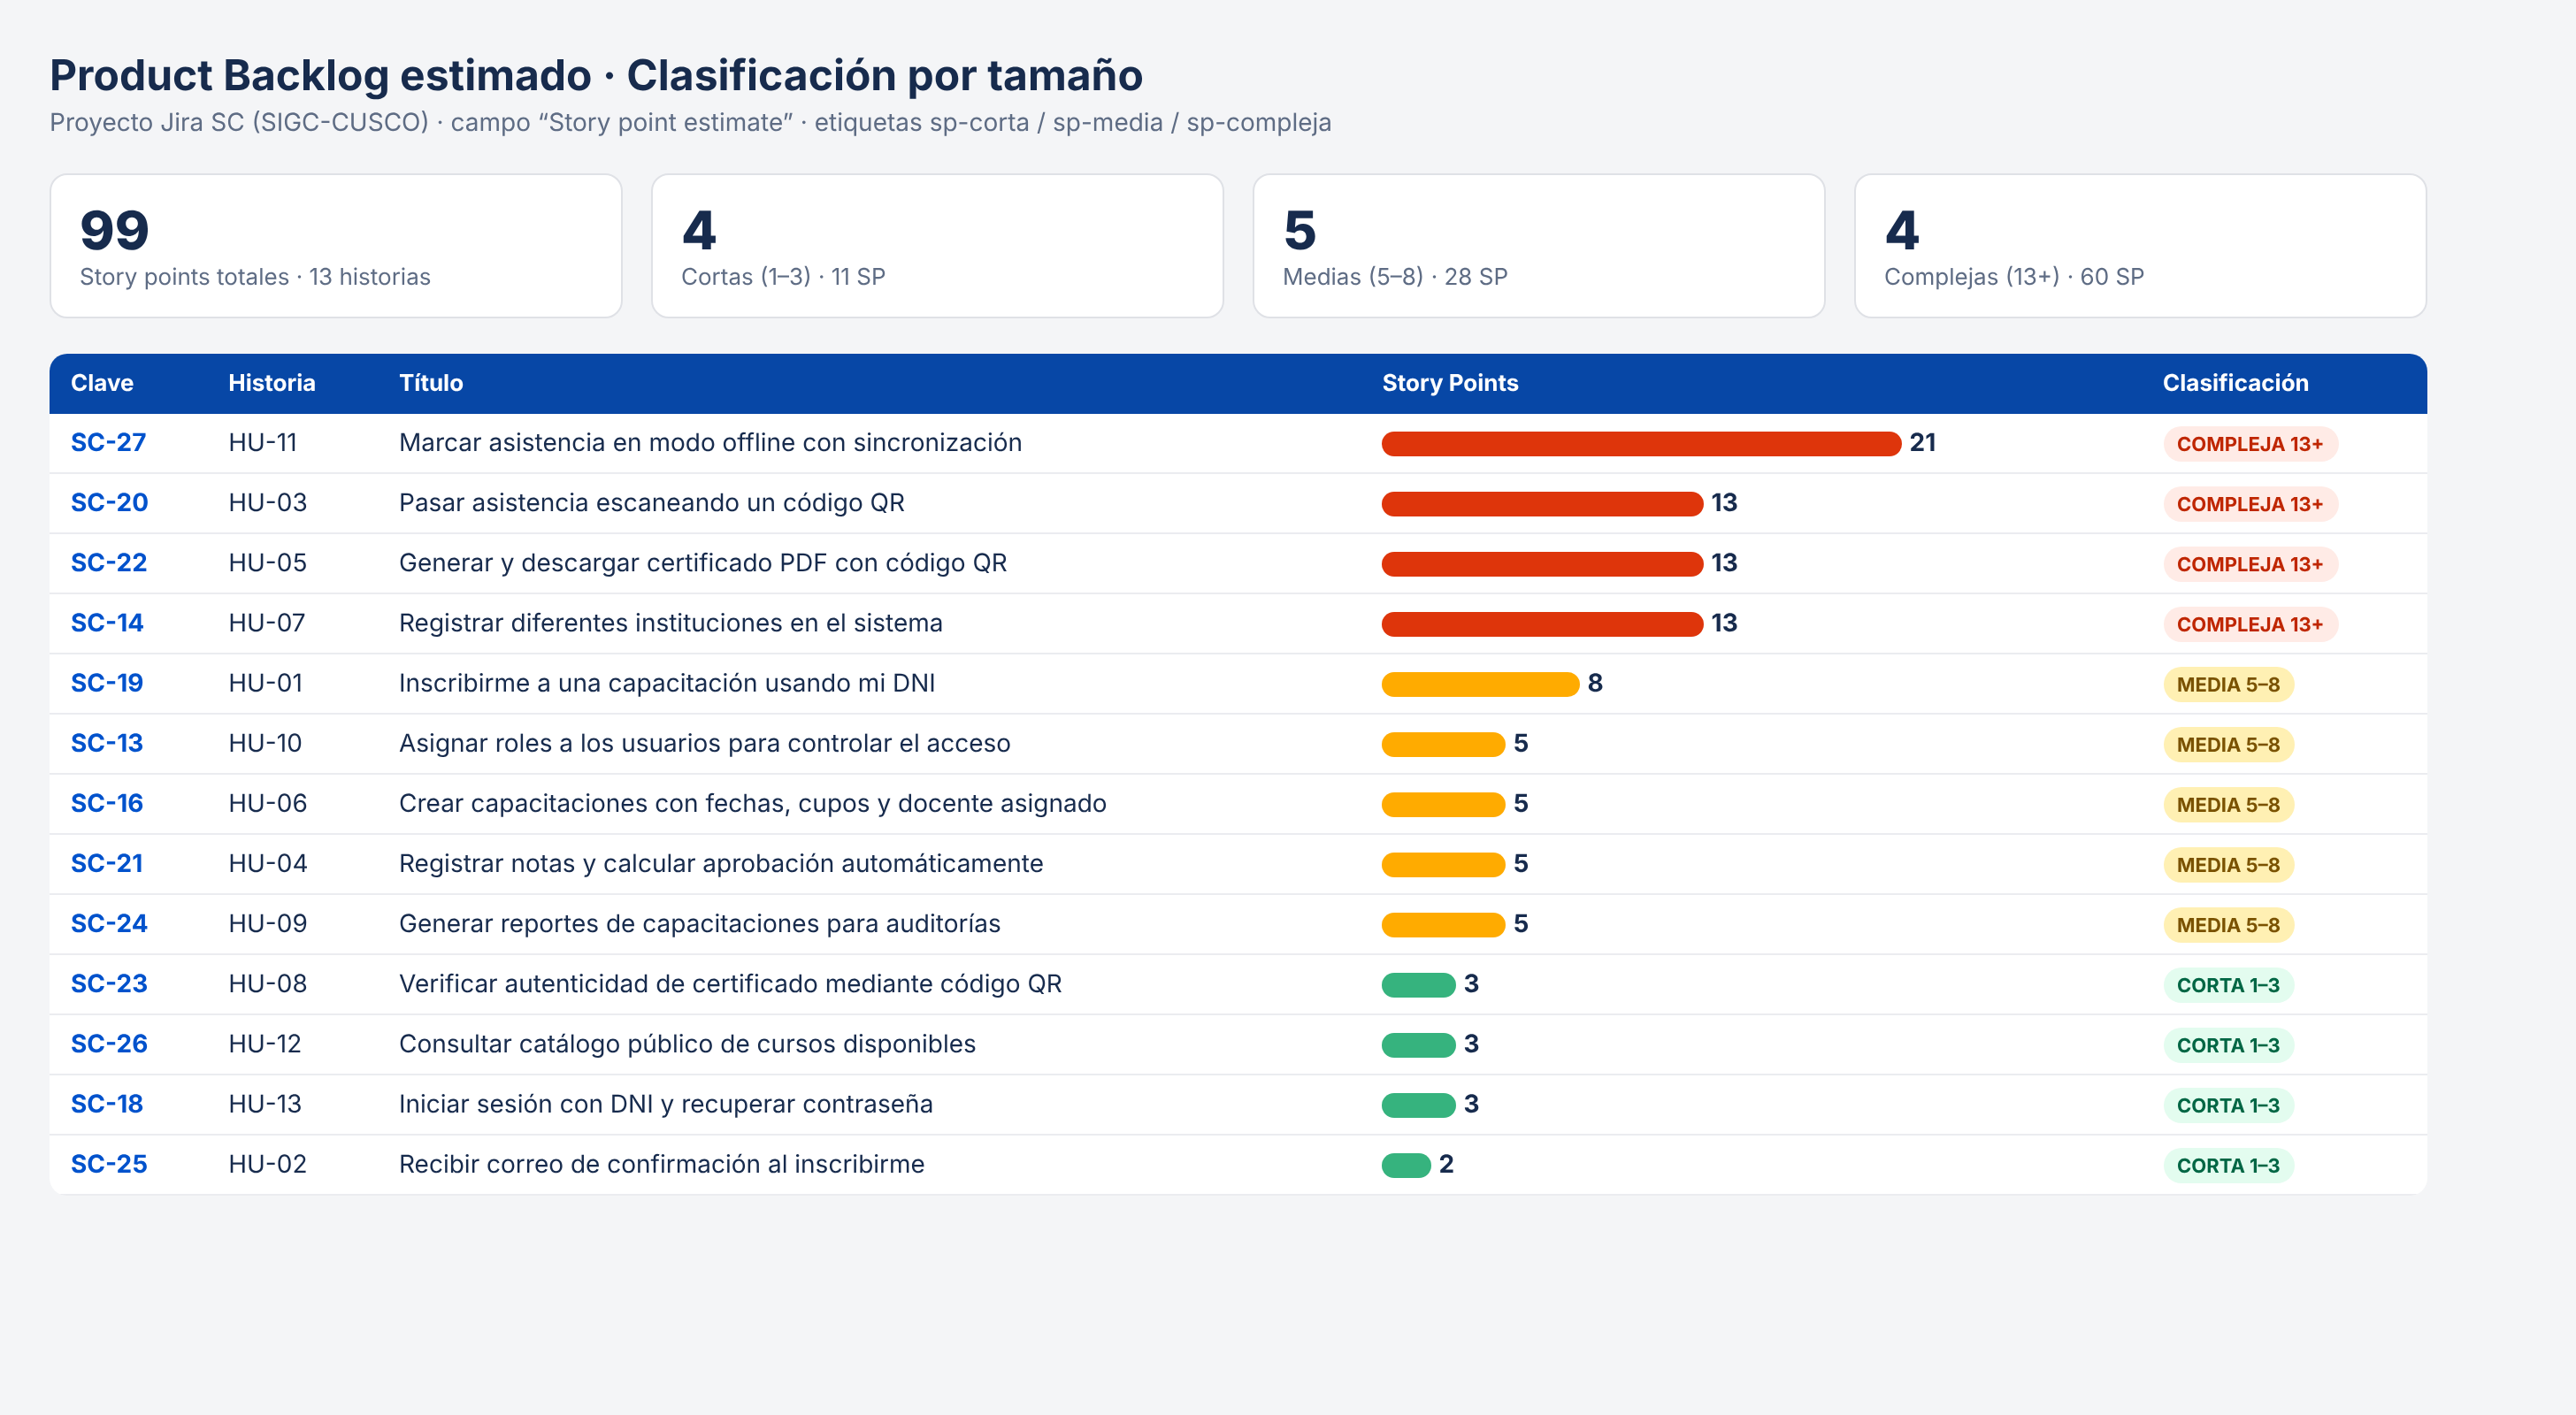
\includegraphics[width=\textwidth]{figura5_backlog_clasificado.png}
    \caption{Visualización ejecutiva del Product Backlog estimado y clasificado por tamaño (Proyecto SC en Jira).}
    \label{fig:backlog_clasificado}
\end{figure}

\subsection{Lectura Analítica y Estrategia de Planificación del Sprint 1}

Una lectura reflexiva de las estimaciones arroja pautas operativas fundamentales para el desarrollo del proyecto:
\begin{enumerate}
    \item \textbf{Carga del núcleo crítico (Must Have):} Las historias clasificadas como \textit{Must Have} totalizan \textbf{49 Story Points}. De ellas, cuatro corresponden a funcionalidades medias (HU-10, HU-06, HU-01 y HU-04, que suman 23 SP), mientras que dos son historias complejas sobredimensionadas (HU-03 y HU-05, sumando 26 SP).
    \item \textbf{Estrategia de ejecución para el Sprint 1:} Sería un error crítico iniciar el desarrollo atacando de golpe las historias de 13 SP. La estrategia idónea consiste en concentrar el primer incremento (Sprint 1) en las historias medias y cortas de cimiento: autenticación y roles (\texttt{HU-13}, \texttt{HU-10}), creación de cursos (\texttt{HU-06}) y el catálogo público con inscripción básica (\texttt{HU-12}, \texttt{HU-01}). Esto permite entregar un sistema funcional de registro mientras en paralelo se refinan y prototipan los componentes de asistencia QR y certificación digital.
    \item \textbf{Disponibilidad de artefactos:} El Product Backlog estimado se encuentra versionado formalmente en el repositorio GitHub en el archivo \texttt{backlog/product\_backlog\_estimado.csv}, garantizando su interoperabilidad con herramientas de reporting automatizado.
\end{enumerate}
